\clearpage
\section{Architektur}
Das ganze System besteht aus verschiedenen Teilen (zum Beispiel der Simulationsserver, der Voter und die Controller) welche
auf bestimmten Arten miteinander kommunizieren und alle eine Funktion erf{\"{u}}llen.

\begin{figure}
	\centering
	\includevisio[width=\textwidth]{Komponenten2}
	\caption{Implementierte Systembestandteile und ihre Beziehungen}
	\label{fig:arch}
\end{figure}


Das Simulationsprogramm besteht aus mehreren Komponenten; deren Funktionalit{\"{a}}t wurde noch weiter in Klassen untergliedert. Allerdings
ist es auf dieser feineren Ebene teilweise sinnvoll Klassen zu bilden die logisch Teile von zweien der Komponenten abbilden. Eine andere
m{\"{o}}gliche Sicht auf das Simulationsprogramm ist daher die Einteilung in zwei Kategorien: als erstes die Klassen die f{\"{u}}r die
Simulation und das Netzwerk zust{\"{a}}ndig sind, als zweites die Klassen die den Benutzer mit dem System interagieren lassen.
\begin{figure}
	\centering
	\includevisio[width=\textwidth]{ClassDiagram}
	\caption{Klassendiagramm}
	\label{fig:uml}
\end{figure}

\subsection{Physiksimulation}
Der wichtigste Teil dieser Bachelorarbeit ist die Simulation. Sie soll nicht nur ein physikalisch glaubw{\"{u}}rdiges Modell
f{\"{u}}r Roboterbewegungen darstellen, den Votern die ben{\"{o}}tigten Informationen zur Steuerung bereitstellen und die
es erm{\"{o}}glichen das empfange Steuerkommandos ausf{\"{u}}hren werden. Dar{\"{u}}ber hinaus soll das Geschehen auch graphisch
dargestellt werden und dem Benutzer die M{\"{o}}glichkeit gegeben werden mit der Simulation zu interagieren, zum einen
durch Bewegen der Kamera, zum anderen durch eine Fernsteuerung eines Roboters (zwecks Fehlerinjektion). Auch diese
Anforderungen wirken sich auf die Implementierung der Physiksimulation aus. 

F{\"{u}}r das Kippen der Platte ist die Klasse PlatePhysics zust{\"{a}}ndig. Sie ist von MonoBehaviour abgeleitet und ist daher
in das Unity Eventsystem eingebunden --- dies erlaubt es innerhalb der Funktion LateUpdate() f{\"{u}}r jeden \textit{\gls{Frame}} den momentanen
Stand der Physiksimulation abzufragen und die Platte entsprechend zu rotieren / kippen.

Der Kippwinkel der Platte wird durch zwei Faktoren bestimmt, das statische und das dynamische Ungleichgewicht. Die Informationen {\"{u}}ber
das statische Gleichgewicht werden von DrawPressureVector() bestimmt. Das dynamische Gleichgewicht wird innerhalb PlatePhysics berechnet,
jeder RobotController {\"{u}}bergibt beim Ausf{\"{u}}hren einer Bewegung diese auch an PlatePhysics. Diese werden dann aufsummiert, ged{\"{a}}mpft
und schlie{\ss}lich zusammen mit dem statischen Gleichgewicht als Plattenrotation / -kippwinkel gesetzt.

Auch f{\"{u}} die Ladestation gibt es eine Klasse, diese erkennt Kollisionen mit anderen Objekten (also den Robotern) und l{\"{a}}dt diese auf
solange der Roboter sich an der Ladestation bedinet.

Eine weitere wichtige Klasse ist RobotController. Um die Roboter zu steueren (ob {\"{u}}ber die manuelle Fehlerinjektion oder mithilfe des
Controllers) und dabei a) das Fehlermodell und b) den physikalischen Status (Ladestatus, momentane Geschwindigkeit, ...) zu beachten. In der
Funktion FixedUpdate, die einmal pro \textit{Frame} aufgef{\"{u}}hrt wird, wird der Roboter bewegt. Dabei n{\"{a}}hrt sich der Roboter den
gew{\"{u}}nschten Beschleunigungen und Rotationen an.

\subsection{Anzeige}\label{graphics}
F{\"{u}}r interessierte Sch{\"{u}}ler und auch f{\"{u}}r die Studenten, die diese Aufgabe l{\"{o}}sen
sollen muss es m{\"{o}}glich sein einzusch{\"{a}}tzen wie der momentane Status der Simulation ist.
Also: wo befinden sich Roboter, wie voll sind sie, wie stark kippt die Platte? All dies soll auch, wie
in \hyperref[anforderung]{Anforderung 5} festgelegt, visuell ansprechend sein.

Da die Unity Engine auch eine vollwertige Grafikengine ist (dies war ja schliesslich ein Kriterium),
kann diese Funktionalit{\"{a}}t genutzt werden. Das Simulationsprogramm ist nicht nur f{\"{u}}r die
reine Simulation sondern auch f{\"{u}}r die Anzeige verantwortlich.

Angezeigt wird eine kreisf{\"{o}}rmige Platte auf der sich die verschiedenen Roboter bewegen. Auch die
Ladestation wird angezeigt.

\paragraph{CameraController} Die Sicht auf die simulierte Welt geschieht durch das Unity Objekt "Camera". An diese
werden verschiedene Skripte angegeh{\"{a}}ngt, um z.B. dem Benutzer die M{\"{o}}glichkeit zu
geben die Kamera zu bewegen und damit einen anderen Teil der Simulation genauer zu betrachten.

Die Kamera kann {\"{u}}ber die Pfeiltasten bewegt werden, ein Kippen der Kamera ist nicht implementiert --
dies w{\"{u}}rde auch verwirren, da damit eventuell der Kippwinkel der Platte visuell ausgeglichen
werden k{\"{o}}nnte. Um immer einen Teil der Simulation im Blick haben zu k{\"{o}}nnen schwebt die Kamera
{\"{u}}ber der Platte und schaut in einem 20\textdegree Winkel schr{\"{a}}g nach unten.

\paragraph{Lichtquelle} Damit etwas sichtbar wird, muss es von Licht getroffen werden. In der Simulation
gibt es daher ein Spotlight. Dies befindet sich weit von der Platte entfernt und scheint in einem steilen Winkel
von links oben auf diese.

\paragraph{Radar} Um einzusch{\"{a}}tzen wie stark die Platte gekippt wurde, k{\"{o}}nnen sich die Studenten einmal
innerhalb der Simulation die Platte anschauen. Um etwas genauer sehen zu k{\"{o}}nen wie die Roboter stehen m{\"{u}}ssten
m{\"{u}}ssten um die Platte ins statische Gleichgewicht zu bringen, wird der momentane Schwerpunkt der Platte visuell
dargestellt.

Dies geschieht durch die Klasse Radar. Sie zeichnet mehrere {\"{u}}berlappende Kreise in die linke, obere Bildschirmecke;
drei der Kreise (Gr{\"{u}}n, Gelb, Rot) symbolisieren die Platte. Auf diesen wird ein schwarzer Kreis gezeichnet, der den
momentanen Schwerpunkt angibt. Anhand der Farbe des Kreises auf welchen der momentane Schwerpunkt liegt ist es sehr einfach
abzulesen wie kritisch der Kippwinkel der Platte, und damit wie gut die Regelung, ist. Und anhand der zweidimensionalen Position
des Schwerpunktindikators k{\"{o}}nnen die Roboter bewegt werden.

\paragraph{FaultInjector\_Player} F{\"{u}}r die Studierenden soll es m{\"{o}}glich sein einen Roboter fernzusteuern um damit
gew{\"{u}}nschte Roboterkonstellationen gezielt herbeizuf{\"{u}}hren. Um anzuzeigen ob die manuelle Fehlerinktion gerade aktiv
oder inaktiv ist wird dem Benutzer, in der Mitte des Bildschirms, dies textuell Text angezeigt.

\subsection{Fehlerinjektion - Physik}
Da es in einer Simulation keine mechanischen (o.{\"{a}}.) Fehler geben kann, das Ziel des Simulationswerkzeuges aber gerade ist
die Studierenden ein fehlertoleranter Systeme entwickelen zu lassen braucht es eine Fehlerinjektion.

Die RobotController konsultieren bevor sie eine neue Zielbeschleunigung und -rotation setzen die Fehlerinjektion {\"{u}}ber den
Status ihres Roboters. Falls beispielsweise einer der Motoren nicht funktioniert hat das Auswirkungen auf die Zielbeschleunigung
(die Richtung und die L{\"{a}}nge des Beschleunigungsvektores werden ge{\"{a}}ndert). Die Informationen {\"{u}}ber den Status
jedes Motoren werden also von der Fehlerinjektionsklasse gespeichert und bereitgestellt.

\subsection{Interface - Simulationsprogramm}
Die Kommunikation zwischen Simulationsprogramm und Voter macht es n{\"{o}}tig das auf beiden Seiten eine Schnittstelle existiert
welche die Kommunikation abstrahiert. Auf der Seite des Simulationsprogrammes wird dies haupts{\"{a}}chlich durch die Klasse
HandleRPCRequests abgehandelt.

An den Voter muss in periodischen Abst{\"{a}}nden der Status der Platte und der sich auf ihr befindenen Roboter gesendet werden.
Daf{\"{u}}r gibt es den pubSock member, eine Instanz der Klasse PublishSocket aus der NNanoMsg Bibliothek. Die andere Aufgabe
dieser Klasse ist es Steuerbefehle der Controller anzunehmen und diese dann an die Roboter weiterzugeben. Daf{\"{u}}r gibt es
den repSock. Beide Aufgaben m{\"{u}}ssen immer wieder ausgef{\"{u}}hrt werden, anstatt einen neuen Thread zu starten werden
nicht-blockierende Funktionen benutzt und sich in das Unityevensystem eingeh{\"{a}}ngt.

\subsection{Interface - Voter}


\clearpage
\section{Fehlerinjektion}
Da es in der Simulation, anders in einer realen Welt, keine normalen Fehlerquellen gibt, wird eine
Fehlerinjektion benutzt, um die Fehlertoleranz zu testen. Die hier simulierten Fehlerarten 
sind im \hyperref[fm]{Fehlermodell} beschrieben.

In diesem Fall wird simuliert, dass das Netzwerk Daten fehlerhaft weiterleitet
(wie es z.B. ein Funknetzwerk tuen w{\"{u}}rde) und das die Controllerprogramme unvorhersehbar
ausfallen - was nachbildet, dass z.B. der Controller seine Batterie entladen hat. Auf der Roboterseite
kann die Funktionsf{\"{a}}higkeit der Motoren eingeschr{\"{a}}nkt werden oder sie k{\"{o}}nnen
falsche Informationen {\"{u}}ber den Status der Welt empfangen.

Wie in \hyperref[anforderung]{Anforderung 3} spezifiert, sind alle Fehlerwahrscheinlichkeiten einstellbar.

\subsection{Netzwerk}
Die Kommunikation zwischen Voter und Controller ist nur {\"{u}}ber ein IP Netzwerk m{\"{o}}glich;
f{\"{u}}r dieses Modul kann ein eigenes Netzwerk aufgebaut werden, in das eine Fehlerinjektionskomponente 
intergiert werden kann. Diese Komponente soll nur die Kommunikation, die von den Studentenprogrammen ausgeht, 
verf{\"{a}}lschen und alle andere normal behandeln. Die St{\"{a}}rke der Fehlerinjektion soll parametresierbar 
sein, zum Beispiel wie wahrscheinlich es ist, das, einzelne Pakete verf{\"{a}}lscht werden oder wie stark
die Verf{\"{a}}lschung sein soll.

Es wird vorgeschrieben, dass die ganze Kommunikation der Studentenprogramme {\"{u}}ber UDP laufen muss. Dadurch reicht es, wenn der Fehlerinjektor nur UDP verf{\"{a}}lscht, was dazu
f{\"{u}}hrt, dass die normalen Administrationstat{\"{a}}tigkeiten nicht beeintr{\"{a}}chtigt werden. Der Fehlerinjektor muss in der Lage sein, mit einstellbaren Wahrscheinlichkeiten
Pakete zu verf{\"{a}}lschen: bei den Arten der Verf{\"{a}}lschung ist es ausreichend, wenn einzelne Bytes gekippt werden.

Daf{\"{u}}r zust{\"{a}}ndig ist Net Inject\cite{kubertzki}. Dabei werden auf den fraglichen Rechnern
Standartrouten definiert, die den Netzwerkverkehr {\"{u}}ber andere Rechner leiten, auf denen Net Inject
installiert ist. Dort werden die Pakete vom Modul NetMod angenommen und es wird {\"{u}}berpr{\"{u}}ft ob
f{\"{u}}r diese Kommunikation (spezifiziert durch Protkoll, Quell- und Zielport) Verf{\"{a}}lschungsregeln
existieren. Anhand dieser Regeln wird das Paket dann ausgwertet und bei Bedarf verf{\"{a}}lscht.

Standardm{\"{a}}ssig ist dieser Fehlerinjektor so eingestellt dass durchschnittlich in $ ^1/_{20} $ aller Pakete ein Byte verf{\"{a}}lscht wird,
ohne dass das Betriebssystem diese Modifikation erkennt. Diese Erkennung muss also von den Studenten selbst implementiert werden.

\subsection{Controller}
Im Fehlermodell wurde spezifiziert, dass die Controller zu beliebigen Zeitpunkten einen
\textit{crash failure} erleiden k{\"{o}}nnen.

Um dies zu erm{\"{o}}glichen, gibt es ein Shellskript, das die Controllerprogramme zu zuf{\"{a}}ligen Zeitpunkten 
beendet und wieder startet - dabei wird das Programm einfach mit SIGKILL beendet und nicht vorgewarnt.
Mit einer Wahrscheinlichkeit von 33\% werden dem Programm auch nur eingeschr{\"{a}}nkte Ressourcen zugeteilt,
z.B. darf es nur eine bestimmte Anzahl an Dateideskriptoren gleichzeitig offen haben oder nur eine 
eingeschr{\"{a}}nkte Menge Speicher benutzen.
\lstinputlisting[language=Bash]{../fault_injector.sh}

\subsection{Simulation}
Auch innerhalb der Simulation soll es Fehler geben, zum Beispiel an den Robotermotoren. Desweiteren soll,
laut Fehlermodell, auch die Fernsteuerung eines Roboters m{\"{o}}glich sein.

Laut \hyperref[fm]{Fehlermodell} k{\"{o}}nnen die Robotermotoren auf verschiedene Arten fehlerbehaftet
sein und die Voter bekommen eventuell fehlerhafte, oder sogar gar keine, Informationen {\"{u}}ber
den Status der Welt. Die Wahrscheinlichkeiten f{\"{u}}r diese verschiedenen F{\"{a}}lle
werden in einer JSON Konfigurationsdatei angegeben. Die Simulation liest diese beim Start aus und 
l{\"{a}}sst dann w{\"{a}}hrend des laufenden Betriebes die Robotermotoren ausfallen.
Ein Teil der Informationen muss an den Voter weitergegeben werden, daher fragt dieser beim Start
automatisch die ben{\"{o}}tigten Daten ab.


\subsubsection{Weltstatus}
Die echten \hyperref[khepera]{Kheperaroboter} haben verschiedene Sensoren (Infrarot, Ultraschall,
odeometrische Motoren, eine Kamera, etc). In der echten Welt k{\"{o}}nnen auch diese Senoren fehlerhaft
sein. Allerdings werden in der Simulation diese Sensoren nicht simuliert, die Roboter kriegen alle
ben{\"{o}}tigten Informationen als Weltstatuspaket. Um die fehlerhafte Sensorik nachzuahmen, soll diese
Informationen abge{\"{a}}ndert werden.

Der Status der Welt der von der Simulation zum Voter geschickt wird kann, wie im \hyperref[fm]{Fehlermodell} angegeben, verf{\"{a}}scht werden, kann zeitweise gar
nicht ankommen oder es kann ein alter Status erneut versendet werden. Die Wahrscheinlichkeiten f{\"{u}}r diese drei F{\"{a}}lle werden direkt angegeben.
\begin{lstlisting}[frame=single, language=json] 
{
	"network" : {
		"dropWorldStatus": 0.001,
		"fakeWorldStatus": 0.001,
		"dupWorldStatus": 0.001
	}
}
\end{lstlisting}

\paragraph{dropWorldStatus} Der Status der Welt kann, aus Sicht des Roboters, einfach nicht ankommen. Dies
	ist ein \textit{omission fault}.
\paragraph{dupWorldStatus} Des weiteren kann ein veralteter Weltstatus ein weiteres Mal empfangen werden.
    Hierbei handelt es sich allerdings immer nur um den jeweils letzten und nicht um noch weiter in
	der Vergangenheit liegende.
\paragraph{fakeWorldStatus} Es ist auch m{\"{o}}glich, dass Daten zur richtigen Zeit ankommen, aber
    verf{\"{a}}lscht wurden. Verf{\"{a}}lscht werden kann hierbei:
	\begin{itemize}
		\item X- und Y-Kippwinkel. Dabei wird einer der Werte um maximal $\pm 2$\textdegree verf{\"{a}}lscht.
			Diese Art der Verf{\"{a}}lschung geschieht in jeweils 40\% der F{\"{a}}lle.
		\item Mit einer Wahrscheinlichkeit von 10\% werden die Daten maximal eines Roboters verf{\"{a}}lscht.
			Namentlich kann hierbei eine der folgenden Daten ver{\"{a}}ndert werden:
			\begin{itemize}
				\item X- oder Y-Koordinaten, um maximal $\pm 5$ Einheiten
				\item Die Rotation, um maximal $\pm 7$\textdegree
				\item Das Gewicht um maximal $\pm 5$ Einheiten
				\item Der Ladezustand um maximal $\pm 50$ Einheiten
			\end{itemize}
			Jede dieser Verf{\"{a}}lschungsarten ist gleich wahrscheinlich, sie liegen also bei 20\%.
		\item Die Daten der Ladestation, nach den gleichen Regeln wie f{\"{u}}r den Roboter
	\end{itemize}

\subsubsection{Motor}
Die zweite Kategorie von Fehlern sind die Ausf{\"{a}}lle der Motoren. Direkt angegeben werden die maximale
Anzahl an fehlerhaften Robotern und die maximale Anzahl an fehlerhaften Motoren pro Roboter.
Die einzelnen Motoren k{\"{o}}nnen entweder tempor{\"{a}}r\footnote{Tempor{\"{a}}r bedeutet
in diesem Fall bis zum n{\"{a}}chsten Steuerbefehl. Dieser wird nat{\"{u}}rlich wieder mit
gleicher Fehlerwahrscheinlich "fehlschlagen"} oder permament fehlerbehaftet (\textit{stuck-at}
oder keinerlei Leitung) sein. Die Wahrscheinlichkeiten f{\"{u}}r diese beiden Fehlerarten werden getrennt
angegeben und k{\"{o}}nnen entweder einer zeitunabh{\"{a}}nigen festen Wahrscheinlichkeit oder der
Badewannenkurve folgen. Bei der Badewannenkurve wird zus{\"{a}}tzlich zur Ausfallwahrscheinlichkeit auch
noch die Dauer (in s) des ersten Bereiches angegeben.
\begin{lstlisting}[frame=single, language=json] 
{
	"robot" : {
		"breakEngineA" : {
			"perm": {"after": 120, "chance" : 0.01}
		},
		"stuckAtEngineA" : {
			"temp": 0.00001
		},
		"maxEnginesBroken": 3,
		"maxEnginesBrokenPerRobot": 1
	}
}
\end{lstlisting}


\subsubsection{Fernsteuerung}
Wie im \hyperref[fm]{Fehlermodell} festgelegt, soll der Benutzer einen Roboter fernsteuern k{\"{o}}nnen
und damit direkten Einfluss auf die simulierte Welt haben. W{\"{a}}hrend ein Roboter ferngesteuert wird, 
f{\"{u}}hrt dieser eine Roboter keine Befehle seines Voters mehr aus. Abgesehen davon verh{\"{a}}lt sich der
Roboter normal, es wird also die gleiche Menge Energie verbraucht, es gelten die gleichen
Einschr{\"{a}}nkungen bei Geschwindigkeit und Rotation, und so weiter.

Dies wird durch ein Script in Unity erm{\"{o}}glicht. Im deaktivierten Zustand zeigt es einen Hilfetext
auf dem Bildschirm an. Mit der Escapetaste wird die Fernsteuerung aktiviert; um dies zu signalisieren wird
der Hilfetext ge{\"{a}}ndert. Dann kann ein Roboter {\"{u}}ber die Pfeiltasten gesteuert werden
(Vorw{\"{a}}rts beschleunigt, Links und Rechts drehen den Roboter). Um anzuzeigen, welcher Roboter
gerade gesteuert wird wird dieser von oben angeleuchtet. Mit der Tabulatortaste kann zwischen den
Robotern umgeschaltet werden. Bei einem weiteren Druck auf die Escapetaste wird die Fernsteuerung deaktiviert.


\clearpage
\section{Die Simulation}
Die simulierte Welt besteht aus den Robotern, die von den Studierenden gesteuert werden sollen, einer Ladestation, an der die Robter Energie tanken k{\"{o}}nnen, und
der Welt, einer kreisf{\"{o}}rmigen, kippbaren Platten, auf der diese Objekte platziert werden und sich bewegen k{\"{o}}nnen.

Simuliert wird die Welt mit der Unity \textit{game engine}. Diese erm{\"{o}}glicht es plattformunabh{\"{a}}nige 
Spiele oder, in diesem Fall, Simulationen zu schreiben. Dabei stellt sie, unter anderem eine Physikengine,
eine Grafikengine und eine Schnitstelle zum Scripten dieser bereit. Desweiteren gibt es auch M{\"{o}}glichkeiten Benutzereingaben
abzufragen, um dem Benutzer die M{\"{o}}glichkeit zu geben mit der Simulation zu interagieren.

Hier werden die M{\"{o}}glichkeiten der objektorierntierten Programmierung genutzt. Jeder Bestandteil der Simulation wird durch
ein Skript abgebildet, diese Skripte k{\"{o}}nnen auch miteinander interagieren. Zum Beispiel benutzt die Robotersteuerungsklasse
die RPC Klasse, so wie dies auch die Fehlerinjektion tut. Genauso wurde die Vererbung genutzt, denn die Roboter und Ladestation haben
einige Eigenschaften gemeinsam (zum Beispiel Position und Gewicht), die eine Vererbungshierachie erm{\"{o}}glichen.

\subsection{Die Roboter}\label{robot}
In der simulierten Welt k{\"{o}}nnen sich bis zu \gls{N} Roboter bewegen. Diese bewegen sich aber nicht selbstst{\"{a}}ndig, sondern werden von den Controllern ferngesteurt.
Wie sie in der Simulation dargestellt werden, wird durch das grafische Modell bestimmt. Anhand dessen bestimmen sich auch die Dimensionen, diese werden f{\"{u}}r die Kollisionerkennung
gebraucht. Die Dimensionen, zusammen mit der Masse, ergeben das physische Modell; dieses hat Auswirkungen auf die Simulation.

\paragraph{Grafisches Modell} Mithilfe von Blender, einem 3D Designprogramm, wurde ein Robotermodell designt, das dem Kepheraroboter\hyperref{khepera} entspricht. Die Grundform des Roboters ist
eine S{\"{a}}ule. Auf dieser befindet sich eine Lampe die den Energielevel angezeigt; daf{\"{u}} {\"{a}}ndert sich ihre Farbe von Gr{\"{u}}n (voll), {\"{u}}ber Gelb bis Rot (leer) .
\todo{Bild}


\paragraph{Physikalisches Modell}
Ein Roboter \gls{Ni} wird dabei beschrieben durch seine Position und Gewicht
$ N_i = \bigl(\begin{smallmatrix} x(i) \\ y(i) \\ w(i) \end{smallmatrix}\bigr)$, eine
Geschwindigkeit $ V_i = \Delta v $ und den momentanen Drehwinkel
$ R_i = r_y(i)$. \todo{Ausdehnung}

Das Gewicht des Roboters ist abh{\"{a}}ngig vom Grundgewicht des Roboters und seinem momentanen F{\"{u}}llstatus: 
\begin{equation}\label{eq:w}
 w(N_i) = 1 + e(N_i) \times 0.03
\end{equation}

Die Roboter haben einen Energiespeicher, der mit maximal 1000 Energieeinheiten
aufgeladen werden kann, und verbrauchen diese Energie, ob beim Fahren oder
Stillstand. Dabei verbrauchen sie pro Sekunde immer eine Energieeinheit und zus{\"{a}}tzlich, abh{\"{a}}ngig von der Geschwindigkeit, Energie f{\"{u}}r die Bewegung:
\begin{equation}\label{eq:entladen}
	e(N_i, t + 1) = e(N_i, t) - 1 - |V_i|
\end{equation}
Falls nicht gen{\"{u}}gend Energie f{\"{u}}r Bewegung und Rotation vorhanden ist, bewegt sich der Roboter nicht.

Die Bewegung des Roboters wird vorgegeben durch $V_l(t)$ und $ V_r(t)$. Diese werden vom Controller, {\"{u}}ber den Voter an die Simulation
weitergegeben und dann von Unity verarbeitet. Die neue Position und der neue Rotationswinkel des Roboters werden errechnet und,
falls gen{\"{u}}gen Energie vorhanden, auch eingenommen - dazu wird der \textit{rigidbody} des Roboters manipuliert.
Um die Bewegung fl{\"{u}}{\ss}iger darzustellen wird zwischen den momentanen und gew{\"{u}}nschten Positionen / Winkel linear interpoliert.

Hierbei muss auch die Fehlerinjektion beachtet werden. Es ist m{\"{o}}glich das die gew{\"{u}}nschte Drehzahl eines Motors nicht eingenommen werden
kann, entweder weil dieser momentan ein \textit{stuck-at}-Verhalten aufweist, oder kaputt (definiert als: Drehzahl = 0) ist. Daf{\"{u}}r wird bevor
die Bewegung durchgef{\"{u}}hrt wird {\"{u}}berpr{\"{u}}ft ob einer der beiden Motoren momentan nicht korrekt funktioniert; ist dies der Fall so wird,
statt des gew{\"{u}}nschten Sollwertes, diesem Motor der Sollwert der Fehlerinjektion zugewiesen. Mit diesem Wert wird nun normal weitergerechnet, also
erst die {\"{U}}berpr{\"{u}}fung ob der Roboter sich von der verbleibenden Energiemenge her so bewegen kann, und -- falls dies der Fall ist -- wird nun
nach und nach diese Drehzahl der Motoren eingenommen was zu einer Rotation und Translation des Roboters f{\"{u}}hrt.

\subsection{Die Ladestation}\label{fuelstation}
Innerhalb der Welt muss eine Ladestation platziert werden, um den Roboter die M{\"{o}}glichkeit zu geben sich aufzuladen. Auch diese wird durch ihren Vektor $ F = \bigl(\begin{smallmatrix} x \\ y \\ w \end{smallmatrix}\bigr)$ beschrieben. Eine Ladestation hat dabei ein festes Gewicht: $ w(F) = 5 $.

Diese wird vor Simulationsbeginn platziert und bewegt sich im weiteren Verlauf nicht.
Falls sich ein Roboter an die Ladestation heranbewegt, also gilt: 
\begin{equation}\label{eq:dist}
 |\bigl(\begin{smallmatrix} x(i) \\ y(i) \end{smallmatrix}\bigr) - \bigl(\begin{smallmatrix} x(F) \\ y(F) \end{smallmatrix}\bigr)| \leq |\bigl(\begin{smallmatrix} 1 \\ 1 \end{smallmatrix}\bigr)|
\end{equation}
wird dieser Roboter aufgeladen. Die Ladefunktion ~\ref{eq:laden} ist hier eine einfache Gerade:
\begin{equation}
    \label{eq:laden}
	e(N_i, t + 1) = max((e(N_i, t) + 10, 1000) 
\end{equation}

\subsection{Die Platte}\label{plate}
Die simulierte Welt besteht aus einer 100 Einheiten gro{\ss}en kreisf{\"{o}}rmigen Platte, die, basierend auf den Gewichten welche sich auf ihr befinden kippt.

Die Kr{\"{a}}fte die auf die Platte wirken berechnen sich nach den Gleichungen \ref{eq:diffs-x}, \ref{eq:diffs-y}. Es wird definiert das die Platte um
maximal 10\textdegree kippen kann; dies sei der Fall wenn die Ladestation und alle Roboter (vollgetankt) am {\"{a}}u{\ss}ersten Rand stehen. Diese theoretisch
m{\"{o}}gliche Maximalkraft entspricht also den 10\textdegree; mithilfe des Dreisatzes ist es nun m{\"{o}}glich die tats{\"{a}}chlichen momentanen Kippwinkel
zu errechnen.

Allerdings wird diese Rechnung erst ausgef{\"{u}}hrt wenn sich 2 (oder mehr) Roboter auf der Platte befinden. Vorher wirkt das Gewicht der Ladestation zu
stark und die Platte ist schon beim Start so stark gekippt das sie nicht mehr ausbalanciert werden kann.

Die Impulse welche auf die Platte wirken (beschrieben in \ref{eq:schwingung}) f{\"{u}}hren zu einer zus{\"{a}}tzlichen Kippung und einer Rotation der Platte.
Immer wenn ein Roboter sich bewegt, wird dieser Bewegungsimpuls gespeichert. Um die momentan auf die Platte wirkenden Kr{\"{a}}fte zu errechnen, werden alle
Impulse aufaddiert. Da der Impuls mit der Zeit abschw{\"{a}}cht wird bei jedem Frame aus dem Anfangsimpuls und der seit dem vergangen Zeit der momentane
Impuls errechnet -- wenn ein Impuls irgendwann keinen sp{\"{u}}rbaren Einfluss auf die Rechnung hat ($ |s(t)| < 0.01$) f{\"{a}}llt dieser Impuls aus der
Rechnung heraus.

Um die Platte dann tats{\"{a}}chlich zu kippen wird die Unity Funktion `AddTorque()` benutzt. Dieser wird ein Kraftvektor {\"{u}}bergeben, um sich also einem
bestimmtem Kippwinkel anzun{\"{a}}hren wird erst die Differenz zwischen den momentanen Winkeln und den gew{\"{u}}nschten errechnet und dann eventuell auf
einen Maximalwert heruntergesetzt (damit die Platte sich langsam zu den gew{\"{u}}nschten Winkeln hinbewegt und nicht direkt "springt"); Dieser Wert kann dann
auf die Platte wirken und rotiert sie in die gew{\"{u}}nschte Richtung.

\subsection{Netzwerkschnittstelle}
Zur Kommunikation mit den Studentenprogrammen gibt es die Netzwerkschnittstelle. Hierr{\"{u}}ber bekommen die Voter die Informationen {\"{u}}ber den momentanen
Status der Welt und k{\"{o}}nnen die Roboter bewegen (nachdem sie einen Roboter erstellt haben). Die Kommunikation geschieht {\"{u}}ber ein selbstentwickeltes
RPC Protokoll. Dieses erlaubt es verschiedene Funktion (aufgef{\"{u}}hrt in \ref{interface}) aufzurufen und die Weltstatusinformationen zu empfangen.

Haupts{\"{a}}chlich verantwortlich hierf{\"{u}}r ist die Klasse HandleRPCRequest. Bei der Initalisierung erstellt sie zwei \textit{sockets}, einen der f{\"{u}}r
die Weltstatusinformationen nach dem \textit{publish-suscribe} Muster sendet (TCP, Port 8001) und einen der die RPC Anfragen bearbeitet (TCP, Port 8000).

In der Update() Funktion werden die Funktion f{\"{u}}r das abarbeiten der RPC Anfragen und das senden der Weltstatusinformationen aufgerufen. In handleRPC()
wird versucht vom socket zu lesen. Dies geschieht nicht-blockierend, so dass, falls keine Daten gelesen werden konnten die Funktion direkt einen Fehler
zur{\"{u}}ckgibt. Ist dies der Fall, passiert in handleRPC() nichts weiter. Sind allerdings doch Daten empfangen worden, werden sie zu allererst deserialisiert.
Danach kann das RPC Paket ausgewertet werden; je nach dem welche Funktion aufgerufen werden soll, verzweigt sich die Ausf{\"{u}}hrung.

Wenn sich ein Voter mit der Simulation verbindet werden als aller erstes die Fehlerinjektionskonfigurationen abgefragt -- dies geschieht durch einen RPC Aufruf
von GET\_FAULT\_INJECTOR\_NETWORK\_CFG. In diesem Fall serialisiert die Simulation diese Daten und schickt sie an den Voter zur{\"{u}}ck.

Als n{\"{a}}chstes erstellt ein Voter einen Roboter, durch Aufruf von CREATE\_ROBOT. In diesem Fall wird aus dem Roboter \textit{prefab} ein Roboter an einer
zuf{\"{a}}lligen Positionen erstellt. Von diesem wird dann die Objektid genommen und an den Voter gesendet. Dieser kann diese nun benutzen um den Roboter zu
steuern.

Die Steuerung eines Roboters geschieht durch einen Aufruf von MOVE\_ROBOT. Dann wird im RoboterController die Funktion MoveRobot() aufgerufen, in der die
Bewegung (unter Beachtung des Ladestands und der Fehlerinjektion) ausgef{\"{u}}hrt wird. Diese RPC Funktion gibt nichts an den Aufrufer zur{\"{u}}ck, Erfolg
oder Misserfolg des Steuerbefehls muss anhand der Weltstatusinformationen erkannt werden.

Wie oft die Weltstatusinformationen (von der Funktion sendWorldStatus()) an alle Subscriber gesendet wird, ist {\"{u}}ber die Konfigurationdateien
einstellbar. Eine genauere Beschreibung des Weltstatus findet sich in \ref{worldstatus}.

\clearpage
\section{Interface f{\"{u}}r die Studenten}\label{interface}
Damit die Studenten sich auf die Implementierung der Fehlertoleranz konzentrieren k{\"{o}}nnen, gibt es Schnittstellen.
Im ganzen System gibt es zwei Schnittstellen:
\begin{itemize}
\item Die Schnittstelle zwischen Controller und Voter
\item Die Schnittstelle zwischen Voter und Roboter/Simulation
\end{itemize}

\paragraph{Die Schnittstelle zwischen Controller und Voter} Den Studenten wird nicht vorgegeben wie die Kommunikation zwischen den Controllern und Votern aussehen soll - denn gerade hier soll ja die Fehlertoleranz implementiert werden.

\paragraph{Die Schnittstelle zwischen Voter und Roboter} Diese Schnittstelle besteht aus den Funktionen:
\begin{lstlisting}[frame=single, language=c] 
void* connectToWorld();
void detachFromWorld(void* ctx);
int createRobot(void* ctx);
typedef void (*TypeGetWorldStatusCallback)(WorldStatus ws, void* optional);
int startProcessingWorldEvents(void* ctx, TypeGetWorldStatusCallback cb, void* optional);
void moveRobot(void* ctx, int id, float vL, float vR);
\end{lstlisting}

Diese wird den Studierenden als kompilierte Library mit einem detailliert kommentierten Headerfile zur Verf{\"{u}}gung gestellt und kann
dann vom Studentencode einfach aufgerufen werden.

Die Weltstatusinformation beschreibt die beiden Kippwinkel der Platte und die Objekte auf dieser. Die Objekte (also Roboter und Ladestation) werden hierbei beschrieben
durch ihre Position, ihre Rotation und Masse. Desweiteren gibt es auch eine eindeutigen Bezeichner und eine Ladestandsanzeige (diese ist allerdings nur bei Robotern
g{\"{u}}ltig).
\label{worldstatus} 
\begin{lstlisting}[frame=single, language=c]
enum SimulationObjectType {
	ROBOT,
	FUEL_STATION
};
typedef struct SimulationObject {
	enum SimulationObjectType type; //! Either "ROBOT" or "FUELSTATION"

	float x; //! x position in the world
	float y; //! y position
	float rotation; //! rotation. 0 < rotation < 360
	float m; //! mass of object

	int id; //! id of this object. Use that for MoveRobot() calls

	int fuel; //! how much fuel that robot has left. invalid for a
		  //! fuel station
} SimulationObject;
\end{lstlisting}

\clearpage
\section{Beispielimplementation}

\todo{20 ist okay, man könnte am Anfang aber nochmal den Bogen zum großen
Bild/Ziel schliessen}

Um das Prinzip dieser Simulation, ob den Studierenden des Moduls Ausfallsichere Systeme oder Besuchern, zu verdeutlichen, ist ein Teil der Bachelorarbeit die Implementierung einer
Beispielimplementation.

\paragraph{Ablauf} Jede Viertelsekunde sendet die Welt Statusinformationen aus. Diese Informationen werden von den Votern empfangen, k{\"{o}}nnen
aber auf dem {\"{U}}bertragungsweg zum Controller potenziel verf{\"{a}}lscht worden sein. Also wird f{\"{u}}r jedes Objekt der Welt der Konsensalgorithmus ausgef{\"{u}}hrt. Wenn ein Konsens {\"{u}ber den Status der Welt hergestellt wurde, berechnet 
jeder Controller f{\"{u}}r jeden Roboter die n{\"{a}}chste Bewegung. Diese wird dann an den Voter geschickt, der ein einfaches Mehrheitsvotum durchf{\"{u}}hrt und diese Bewegung an die Welt weitergibt.

\subsection{Fehlermodell} \label{error-model}
Bei der Planung eines ausfallsicheren Systems ist es besonders wichtig zu definieren, welche Art von Fehlern
{\"{u}}berhaupt korrigiert / abgefangen werden soll. F{\"{u}}r die Beispielimplementation ist es nicht
n{\"{o}}tig eine Regelung zur Ausbalancierung zu entwickelen. Daher werden nur f{\"{u}}r bestimmte Fehlerklassen
die m{\"{o}}glichen Fehler aufgelistet und beschrieben, ob und wie sie gel{\"{o}}st werden.

\paragraph{Crash failure} Die Controller k{\"{o}}nnen jederzeit ausfallen. Im Extremfall k{\"{o}}nen alle Controller ausfallen, die Voter sind, per Definition, gegen diese Art von Fehlern unempfindlich.

\paragraph{Value error} Das Netzwerk kann Pakete verf{\"{a}}lschen, es wird angenommen, dass bei bis zu
$^1/_{20}$ aller Pakete Verf{\"{a}}lschungen geben kann, diese sich allerdings auf
\textit{Single Byte Errors} beschr{\"{a}}nkt. Dar{\"{u}}ber hinausgehende Verf{\"{a}}lschungen werden nicht
erkannt und f{\"{u}}hren zu einem \textit{silent failure}; Dadurch wird der Roboter fehlerhaft angesteuert,
dies ist allerdings nicht mehr Teil des Fehlermodells.

\subsubsection{R{\"{a}}umliche Redudanz}
Es wird davon ausgegangen, dass die Controller sehr fehleranf{\"{a}}llig sind und leicht ausfallen --
daraus folgt das eine gro{\ss}e Anzahl ($Y$) an Controllern f{\"{u}}r jeden Roboter kontrollieren muss;
nur falls weniger als $X$ Controller dieses Roboter noch aktiv sind kann eine ordnungsgem{\"{a}}{\ss}e
Steuerung nicht mehr garantiert werden. Zu bestimmen wie gro{\ss} $X$ sein muss ist nicht Teil der
Beispielimplementation.

\subsubsection{Netzwerkkommunikation}
Da durch die Fehlerinjektion das Netzwerk UDP Pakete verf{\"{a}}lscht, m{\"{u}}ssen alle Daten mit einer 
Kanalkodierung versehen werden. Hier wird ein (255, 240) Reed-Solomon Code benutzt, also ein Code, der 15 parity 
bits pro 240 Datenbits benutzt. Durch die Benutzung dieser Kodierung k{\"{o}}nnen alle Einzelfehler und 
Doppelfehler erkannt und korrigiert werden. Erst ab 7 Fehlern ist eine Korrektur nicht mehr m{\"{o}}glich, ab 15 
Fehlern versagt auch eine Fehlererkennung.

Diese Kodierungsart wurde aus zwei Gr{\"{u}}nden gew{\"{a}}hlt:
\begin{itemize}
\item Durch expermientelle Verifikation wurde klar, dass im Netzwerk nur 1 Byte pro Paket verf{\"{a}}lscht wird.
	Da das durchschnittliche Paket um mindestens Faktor 100 gr{\"{o}}{\ss}er ist, ist nicht erforderlich,
	eine sehr kompakte Kodierung zu benutzen, es ist ausreichend, die Redudanz zu reduzieren. 
\item Es ist ein systematischer Code, der es erlaubt, w{\"{a}}hrend des laufenden Betriebes die Pakete 
	mitzuschneiden und sich die Daten anzugucken. Dies vereinfacht die Fehlersuche -- beispielsweise bei
	einem Viterbicode w{\"{a}}re dies nicht m{\"{o}}glich, dort sind Nutz- und Kodierungsdaten nicht klar 
	unterscheidbar.
\end{itemize}

\subsection{Voter}
\label{voter}
Der Roboter kann nur direkt durch den Voter gesteuert werden. Der Voter ist dabei nur daf{\"{u}}r
zust{\"{a}}ndig, aus den vielen Steuerkommandos, die ankommen, die Mehrheit zu bilden (\textit{N-modular reduancy}).
Da nicht klar ist, wie viele Controller momentan {\"{u}}berhaupt Steuerkommandos senden k{\"{o}}nnten,
kann nicht gewartet werden bis eine bestimmte Anzahl von Kommandos empfangen wurde. Deswegen wird beim Empfangen
eines neuen Weltstatus (also zu periodisch wiederkehrenden Zeitpunkten) das Steuerergebniss gebildet,
weggesendet und der Vorgang wird neu gestartet.

Um das Steuerergebniss zu finden werden die empfangenen Steuerkommandos sortiert und der Medianwert genommen 
(\textit{Mid-Value Selection}). Anstatt des Mittelwerts wird der Medians genutzt weil dadurch weniger "extreme"
Bewegungen bevorzugt werden.
\noindent\begin{minipage}{.30\textwidth}
	\begin{lstlisting}[caption=Sammeln, frame=tlrb, language={[11]C++}]
votes.res[id].push_back(Vector{x, y});
\end{lstlisting}
\end{minipage}\hfill
\begin{minipage}{.60\textwidth}
\begin{lstlisting}[caption=Auswahl, frame=tlrb, language={[11]C++}]
/* go through all robots */
for(auto&& votes : votes.res) {
  /* vote */
  std::sort(std::begin(votes.second), std::end(votes.second));
  auto x = votes.second[votes.second.size() / 2];

  /* send */
  int r = 0;
  if((r = moveRobot(info->worldCtx, votes.first, x.x_, x.y_)) < 0) {
  	fprintf(stderr, "can't move robot: %d", r);
  }
}
\end{lstlisting}
\end{minipage}


\begin{figure}
	\centering
	\includevisio[width=\textwidth]{seqvoter}
	\caption{Ablaufdiagramm Voter}
	\label{fig:sequence-voter}
\end{figure}
\clearpage % make sure the table is, at least, in the right section

\subsection{Controller}\label{controller}
Die Roboter m{\"{u}}ssen sich so bewegen, dass die Platte m{\"{o}}glichst gut ausbalanciert
ist und gleichzeitig die Roboter nicht ihre ganze Tankf{\"{u}}llung verbrauchen. Gleichzeitig sollten
die Roboter auch nicht miteinander kollidieren.

\paragraph{Algorithmus zur Bestimmung der Bewegung} Der implementierte Algorithmus unterschiedet zwischen 3 Situation: ist der Zustand des Roboters kritisch,
unkritisch oder dazwischen? Dabei ist das Kriterium die momentane Tankf{\"{u}}llung geteilt durch die Entfernung zur Ladestation. Roboter mit fast leerem Tank
versuchen also sich aufzuf{\"{u}}llen, Roboter mit fast vollem Tank versuchen auszubalancieren.

Jeder Controller berechnet f{\"{u}}r jeden Roboter wie dieser sich bewegen soll. Dabei wird mit dem Roboter
im kritischtesten Zustand anfangen, denn dieser muss ja unbedingt Richtung Ladestation gesteuert werden 
und die weniger kritischen k{\"{o}}nnen/m{\"{u}}ssen diese Bewegung dann ausgleichen. Daf{\"{u}}r werden nach
jeder berechneten Roboterbewegung die Weltkippwinkel neu berechnet, so dass die vollsten Roboter die Bewegungen
der vorher berechneten mit in ihre Entscheidung einbeziehen.


Um nun zu einem Punkt zu fahren wird sich anhand des Drehwinkels gedreht und entsprechend des Distanzvektores 
bewegt. Rotation und Translation werden nacheinander ausgef{\"{u}}hrt. Dies ist zwar langsamer, erleichtert die
Implementierung aber ungemein.

\paragraph{Ausbalancieren} Auch das ausbalancieren kann als Bewegung zu einem Punkt aufgefasst werden.
Die Platte ist ja durch die Gewichte der Roboter aus dem Gleichgewicht gebracht worden, um sie wieder ins
Gleichgewicht zu bringen k{\"{o}}nnten sich die einzelnen Roboter ja an den jeweiligen Punkt bewegen der
die Platte ins Gleichgewicht bringen w{\"{u}}rde.

Dazu wird zuerst der Kippwinkel der Platte ohne den momentan betrachteten Roboter berechnet. Anhand dessen
kann bestimmt werden an welcher Position der momentan betrachtete Roboter sein m{\"{u}}sste um die Platte
ins Lot zu bringen. Dorthin bewegt der Roboter sich nun, stoppt allerdings am Rande der Platte um nicht
herunterzufallen -- schlie{\ss}lich kann es sein das dieser Roboter sich von der Platte bewegen m{\"{u}}sste
um die Platte auszubalancieren.

\clearpage
\section{Zusammenfassung}
Das Ziel dieser Bachelorarbeit war die Entwicklung einer {\"{U}}bungsaufgabe um Studierenden der Fachhochschule
S{\"{u}}dwestfalen die Grundz{\"{u}}ge der Ausfallsicheren Systeme beizubringen. Dabei soll die schon bestehende
{\"{U}}bungsaufgabe\ref{heizung} erg{\"{a}}nzt werden.

Dabei besteht das System aus mehreren Teilen. Zum einen das Simulationsprogramm das gleichzeitig auch als
Server f{\"{u}}r die, von den Studenten zu programmierenden, Roboter fungiert. Die Roboter bestehen aus
einem von den Studierenden programmierten Teil; dieser benutzt die libworld um sich mit der Simulation zu
verbinden und die Roboter in ihr zu steuern.

Da das Hauptziel des Simulationswerkzeuges war den Studenten eine weitere {\"{U}}bungsaufgabe zur Verf{\"{u}}gung
zu stellen, ist das Hauptbewertungskriterium wie gut diese Simulation f{\"{u}}r diesen Zweck geeignet ist.

Die anderen Kriterien sind: \todo{}

\begin{enumerate}
	\item Die Alternativaufgabe soll sich stark von der ausfallsicheren Heizung unterscheiden, damit die Studierenden eine tats{\"{a}}chliche Wahl haben.
	\item Um die Aufgabe zu l{\"{o}}sen, muss eine Vielzahl von Konzepten der Ausfallsicherheit genutzt werden.
	\item Es soll visuell ansprechend sein.
	\item Es darf auch durch unsachgem{\"{a}}ssen Gebrauch nicht gesch{\"{a}}digt werden
\end{enumerate}

Es ist allerdings m{\"{o}}glich auszuwerten ob die anderen Anforderungen erf{\"{u}}llt worden sind. Als erstes
soll hier die M{\"{o}}glichkeit betrachtet werden (im Gegensatz zur Heizung) das mehrere Gruppen gleichzeitig
an ihrer L{\"{o}}sung arbeiten k{\"{o}}nnen. Durch die Nutzung eines Servers zu dem sich die Voter/Roboter
verbinden zusammen mit ein wenig Absprache der Gruppe kann dieses Ziel erreicht werden. Die Simulation welche
auf diesem Server l{\"{a}}uft liest beim Start eine Konfigurationdatei ein, mit der verschiedene Einstellungen
der Fehlerinjektion frei gew{\"{a}}hlt werden k{\"{o}}nnen.

Mithilfe der Beispielimplementation (und einigen speziellen Testprogrammen) ist es m{\"{o}}glich einen Systemtest
durchzuf{\"{u}}hren. Bei einem Systemtest werden die Komponenten nicht seperat voneinander getestet, sondern das
gesamte System wird gleichzeitig getestet. Diese Art von Tests verifiziert das Zusammenspiel der Komponenten.

Die Aufgabe welche von den Studierenden zu bew{\"{a}}ltigen ist, ist es die Platte so gut wie m{\"{o}}glich zu
stabilisieren und dabei m{\"{o}}gliche Fehler zu erkennen und so gut wie m{\"{o}}glich zu beheben. Es muss also
ein physikalisches und ein informationstechnologisches Problem gel{\"{o}}st werden. Daher sollte das System in
Bezug auf die Anforderungen im Hinblick auf die Korrektheit der physikalischen Simulation und der korrekten
Funktionalit{\"{a}}t der Fehlerinjektion getestet werden.

\subsection{Evaluierung in Bezug auf Lernziel}
Wie sehr diese Bachelorarbeit als Lehrmittel zeigt, kann noch nicht evauliert werden. Dies wird erst w{\"{a}}hrend
der Benutzung durch die Studenten ersichtlich.

\subsection{Evaluierung in Bezug auf Simulation - Physik}
Die Physiksimulation simuliert Roboterbewegungen, das Entladen der Roboter und das Kippen der Platte. Diese k{\"{o}}nnen
seperat getestet werden.

Das Bewegungsmuster der Roboter ist an den \textit{differential drive}\ref{diff} angelehnt. Dazu wird f{\"{u}}r den ersten Test ein
Roboter nach festen Regeln bewegt. Durch die spezifischen Begebenheiten des \textit{differential drive} gibt es beispielsweise die einfachen
Bewegungsmuster:
\begin{enumerate}
	\item Eine Bewegung gerade nach vorn
	\item Eine Bewegung gerade nach hinten
	\item Eine Rotation auf der Stelle (im Uhrzeigersinn)
	\item Eine Rotation auf der Stelle (gegen den Uhrzeigersinn)
\end{enumerate}

Aus diesen k{\"{o}}nnen sich weitere Bewegungsarten zusammensetzen. Um zu testen ob in der Simulation die Bewegungsarten korrekt implementiert
wurden, werden die abgefahren Wege f{\"{u}}r diese aufgezeichnet und mit den erwarteten Wegen verglichen.
\begin{figure}
\centering
\begin{subfigure}{.5\textwidth}
  \centering
  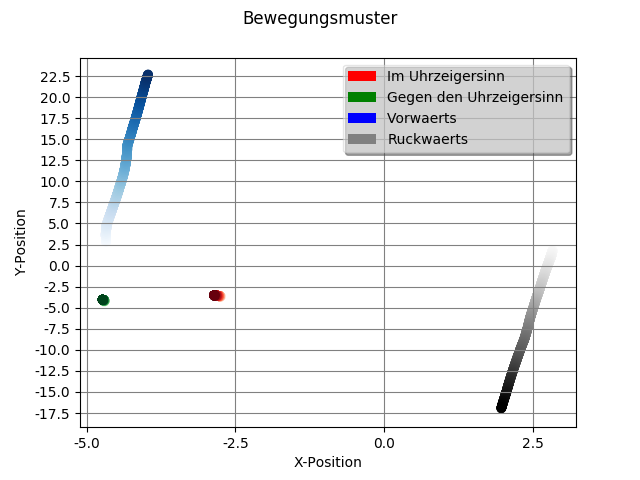
\includegraphics[width=.4\linewidth]{bewegungsmuster_simpel}
  \caption{Die Grundbewegungsarten}
  \label{fig:move1}
\end{subfigure}%
\begin{subfigure}{.5\textwidth}
  \centering
  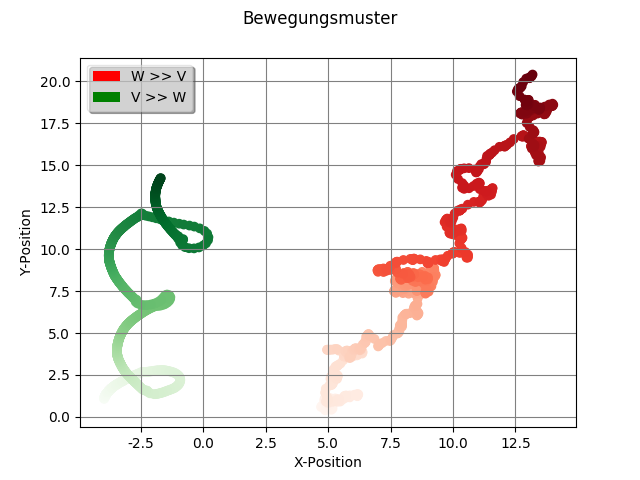
\includegraphics[width=.4\linewidth]{bewegungsmuster_kombi}
  \caption{Kombinierte Bewegungsarten}
  \label{fig:move2}
\end{subfigure}
\caption{Verschiedene Bewegungsarten}
\label{fig:move}
\end{figure}

Es wird ersichtlich das bei der Roatation auf der Stelle es f{\"{a}}lschlicherweise kleinere Bewegungen gibt. Diese sind auch bei den reinen
Bewegung nach vorne und hinten erkennbar. \todo{ka ob die kombinierten richtig sind. waren jedenfalls 200 100 und 100 200}

Ein weiterer Testfall ist ob die Bewegungen des Roboters zu einem Entladen f{\"{u}}hren. Daf{\"{u}}r wurde ein Testprogramm geschrieben
das den Roboter mit einer festen Geschwindigkeit {\"{u}}ber die Platte fahren l{\"{a}}sst und sich beendet sobald der Roboter sich
entladen hat. Anhand der Durchlaufzeit des Programmes und der vorgegebenen Geschwindigkeit (und damit des erwarteten Verbrauches
laut Formel \ref{eq:entladen}) ist es m{\"{o}}glich den tats{\"{a}}chlichen Verbrauch herauszufinden.

\todo{durchfuehrung. am coolsten waere ein balkendiagramm, x achse sind 3 Geschwindigkeit, dann jeweils ein Balken fuer errechnet
und gemessen}

Da in der Simulation die Roboter sich nicht nur entladen sollen, sondern m{\"{o}}glichst lange fahren sollen gibt es eine
Ladestation welche die Roboter aufl{\"{a}}dt falls diese nah genug an dieser sind. Es ist m{\"{o}}glich ein Testprogramm zu
schreiben welches den Roboter an die Ladestation heranf{\"{a}}hrt und dort stehen bleibt. Die Roboter haben einen bestimmten
Grundumsatz der nach 1000 Sekunden\footnote{Bei einem Grundumsatz von 1 pro Sekunde und keinerlei Bewegung}
dazu f{\"{u}}hren w{\"{u}}rde das der Roboter seine Energie verbraucht hat. Falls der Roboter allerdings
konstant aufgeladen wird, sollte dieser Roboter sich auch nach viel l{\"{a}}ngere Zeitspannen nicht entleeren.
\begin{subequations}\label{eq:eval:laden}
\begin{align}
 e_i(t = 0) = 1000
	e_i(t = X) = 1000 - 1 * X  = 0 \\
	\implies e_i(t = 1000) = 0
\end{align}
\end{subequations}


\todo{durchfuerung, vlt einfach diagramm mit fuellstatus ueber zeit?}

\subsection{Evaluierung in Bezug auf Simulation - Fehlerinjektion}
Da die Fehlerinjektion die Fehler zuf{\"{a}}llig injeziert ist eine statistische Auswertung notwendig. Das hei{\ss}t praktisch das
der gleiche Versuch mehrmals ausgef{\"{u}}hrt werden muss und der Anteil der "gegl{\"{u}}ckten" Versuche mit dem Erwartungswert
verglichen wird.

F{\"{u}}r den ersten Test wird die Fehlerinjektionswahrscheinlichkeit f{\"{u}}r den Motor A einmal von (ann{\"{a}}hrend) null immer
weiter erh{\"{o}}ht. Falls die Fehlerinjektion wirkt, also der Motor immer wieder mal tempor{\"{a}}r ausf{\"{a}}llt sollte die
Zeit um eine Strecke abzufahren proportional mit der Fehlerinjektionswahrscheinlichkeit steigen.
\footnote{In diesem Fall wurden 4 Messdurchg{\"{a}}nge aufgezeichnet und nur der Mittelwert der ersten 60s gezeigt.}

\begin{figure}
	\centering
	\includevisio[width=\textwidth]{zemsf}
	\caption{Zur{\"{u}}ckgelegte Entfernung mit steigender Fehlerwahrscheinlichkeit}
	\label{fig:}
\end{figure}


